%Preambulo
\documentclass[12pt]{article}
\usepackage[utf8]{inputenc}
\usepackage[spanish]{babel}
\usepackage{geometry,graphicx}

%Tamaño de Hoja y Márgenes del Documento
\geometry{letterpaper, left=2cm,right=2cm,top=2cm,bottom=4cm}


%Inicio del documento
\begin{document}
	%Portada
	\begin{titlepage}
		\centering
		\textbf{\LARGE Universidad de Costa Rica}\\
		\vspace{3cm}
		\textbf{\Large Ingeniería Eléctrica}\\
		\vspace{1.5cm}
		\textsc{ \Huge Proyecto:}\\
		\vspace{3cm}
		\textit{\Large Pokédex en Javascript }\\
		\vfill       
		\Large Autor: \\
		\Large Jason Antonio Luna Vega\\
		\vfill
		\Large Octubre 2023\\
	\end{titlepage}
	
	\tableofcontents\vspace{18cm}

    \section{Introducción: }
    En este documento se detallará el proyecto de programación que se desarrollará para este curso, el cual consiste en crear una aplicación web basada en una pokédex la cual es un sistema creado en el mundo de pokémon para poder llevar un inventario de la cantidad de pokémones capturados a lo largo del juego.También se añadiran funciones para busqueda por nombre,tipo o generación de pokemons,una pestaña que realizara una comparación de dos pokemons e imprimira el posible ganador de un combate entre estos 2. Y por ultimo una página que mostrará la tabla de debilidades y fortalezas de cada tipo de pokemon.\vspace{0.5cm}
    \\
    Para este proyecto se hará uso de tecnologías como HTML,CSS,JavaScript,Github,GithubPages y la API de PokéApi de cual se extraerá la información de cada uno de los pokémones que se podrán consultar en la aplicación.\vspace{0.5cm}
    \\

    \section{Objetivos: }
        \begin{itemize}
            \item Objetivo General: Desarrollar una aplicación web en JavaScript basada en el sistema de Pokédex donde los usuarios puedan consultar la información de los pokémons por nombre, tipo, región y generación.
            \item Objetivos Especificos:
                \subitem Implementar un API en la aplicación que facilite la obtención de datos.
                \subitem Desplegar la aplicación para el uso del publico.
                \subitem Implementar un sistema de control de versiones para el desarrollo de la aplicación.
        \end{itemize}

    \section{Alcances:}
        \begin{itemize}
            \item Aplicación funcional.
            \item Amigable con el usuario.
            \item Interfaz facil de usar.
            \item Acceso al público.
            \item Despliegue vía web.
            \item Manejo correcto de la información.
            \item Diseño responsivo.
        \end{itemize}

    \section{Justificación: }
    El motivo del desarrollo de este proyecto es debido a que siempre me ha gustado este tipo de juegos pero es un poco molesto tener que capturar los pokémons para visualizar su información o saber a que posición de la pokédex pertenece un pokémon por lo que lo mas convencional es tener un sistema donde se pueda consultar los datos de cada uno sin necesidad de tener que capturarlos dentro del juego.\vspace{0.5cm}
    \\
    De esta forma los usuarios pueden tomar mejores decisiones a la hora de formar su equipo dentro del juego cuales son los pokémons que mas les convienen o que mas les gusten. También saber donde se encuentra cada uno de estos dentro del juego, saber su tipo y demás detalles que son importantes a la hora de avanzar en la historia del juego.\vspace{0.5cm}
    \\

    \section{Marco Teórico: }
        \subsection{Antecedentes:}
            Este es un proyecto desarrollada anteriormente por multiples personas por lo cual se cuenta con una amplia variedad de ejemplos de los cuales se tomarán como referencia para la realización de este sistema esto no quiere decir que se vaya a copiar de un ejemplo especifico si no usar todas estas referencias para desarrollar una aplicación que cumpla con los objetivos ya descritos anteriormente.
        \subsection{Problema:}
            El problema que se quiere desarrollar y resolver es el proceso tardado de cada usuario al estar jugando un juego de pokémon y tener que capturar cada uno de los pokémons para obtener la información de cada uno de ellos lo cual es un proceso muy tardado, con el sistema de pokédex se quiere facilitar esta labor a los entrenadores y de esta forma ellos puedan encontrar los pokémons que mas les convenga para su aventura.
        \subsection{Requisitos del proyecto: }
            \begin{itemize}
                \item Debe permitir a los usuarios consultar los pokémons por su nombre, tipo y generación.
                \item Capacidad de ayudar al usuario en las elecciones de su equipo con metodos de comparación de tipos y pokemons.
                \item Interfaz amigable para el usuario y que pueda ser utilizada en cualquier dispositivo.
                \item Acceso al público en general para el uso del sistema.
            \end{itemize}
            \vspace{3cm}
        \subsection{Estructura del proyecto: }
            \begin{itemize}
                \item Capa de presentación: Esta capa se encargará de mostrar la interfaz de usuario del sistema. Estará construida con HTML, CSS y JavaScript.
                \item Capa de procesamiento de datos: Esta capa se encargará de procesar las peticiones de los usuarios y devolver la información correspondiente. Estará construida con JavaScript.
                \item Capa de despliegue: Esta capa es la encargada de desplegar el proyecto vía web y permite ser accesible a cualquier usuario que quiera utilizar el sistema.
            \end{itemize}
        \subsection{Metodología de desarrollo: }
        El proyecto se desarrollará utilizando la metodología de desarrollo ágil. Esta metodología se basa en el desarrollo iterativo e incremental, lo que significa que el sistema se irá construyendo por partes, de forma que se pueda ir evaluando su progreso a medida que se desarrolla.
        \subsection{Tecnologías: }
        El proyecto se desarrollará utilizando las siguientes herramientas y tecnologías:
        \begin{itemize}
            \item HTML: El lenguaje de marcado para la estructura de la página web.
            \item CSS: El lenguaje de hojas de estilo para el diseño de la página web.
            \item JavaScript: El lenguaje de programación para la lógica del sistema.
            \item ReactJS: Una biblioteca de JavaScript para la creación de interfaces de usuario.
            \item GitHub: Un sistema de control de versiones para el seguimiento del código.
            \item GitHub Pages: Un servicio de alojamiento web para la publicación de proyectos de GitHub.
        \end{itemize}
        \subsection{Limitaciones:}
        \begin{itemize}
            \item Problemas con implementación de Frameworks.
            \item Falta de conocimiento de estilos en CSS.
            \item Aplicación con carga lenta debido a no usar Frameworks para la administración de las páginas y elementos de la aplicación.
            \item Ordenamiento por generaciones.
        \end{itemize}
    \section{Desarrollo:}
        \subsection{Página principal:}
        La pagina principal de el proyecto es una serie de cartas ordenadas de manera ascendente con el contenido mas impotante de cada pokemon(nombre,numero,tipo) cada carta generada posee un color dependiendo del tipo de pokemon y están generadas desde la generación 1 hasta la generación 8 incluyendo megaevoluciones.
        \begin{figure}[h]
            \centering
            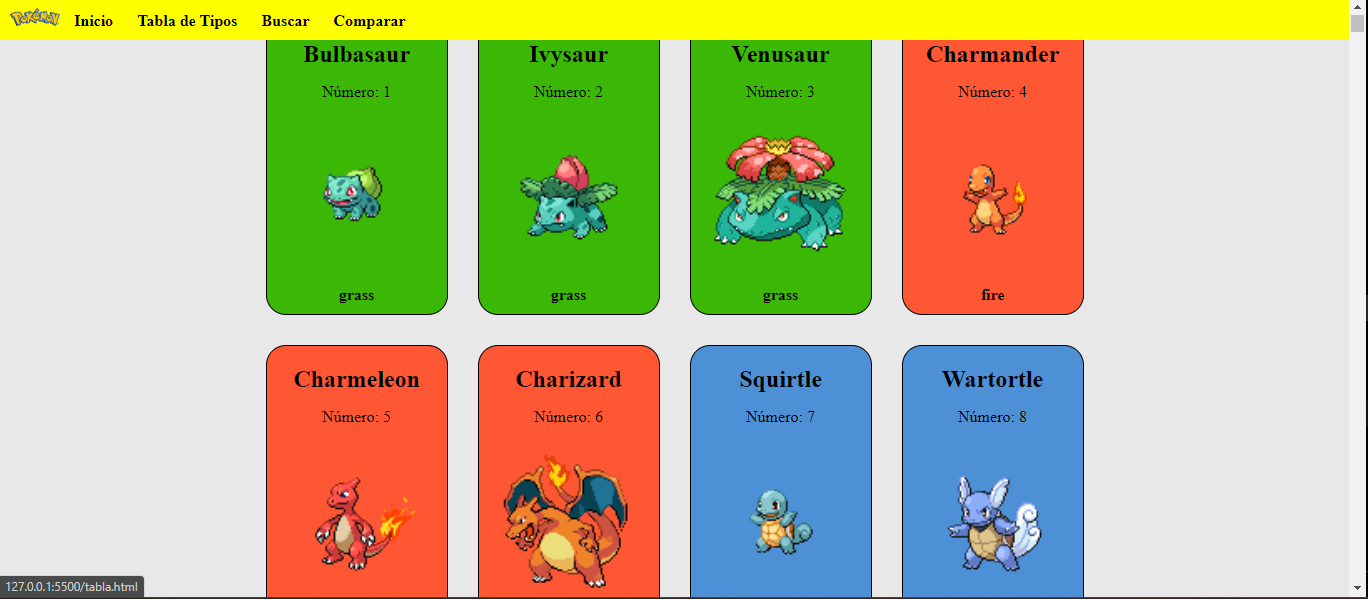
\includegraphics[width=0.5\textwidth]{img/homepage.png}
            \caption{Pagina Principal}
            \label{figure:homepage}
        \end{figure}

        \subsection{Página Tabla de Tipos:}
        Este apartado de la aplicación genera en formato de tabla las fortalezas y debilidades de cada tipo de pokemon lo que le permite al usuario saber en un combate cual pokemon debería utilizar contra el tipo al que se esta enfrentando y pueda hacerle daño x2 o x4.
        \begin{figure}[h]
            \centering
            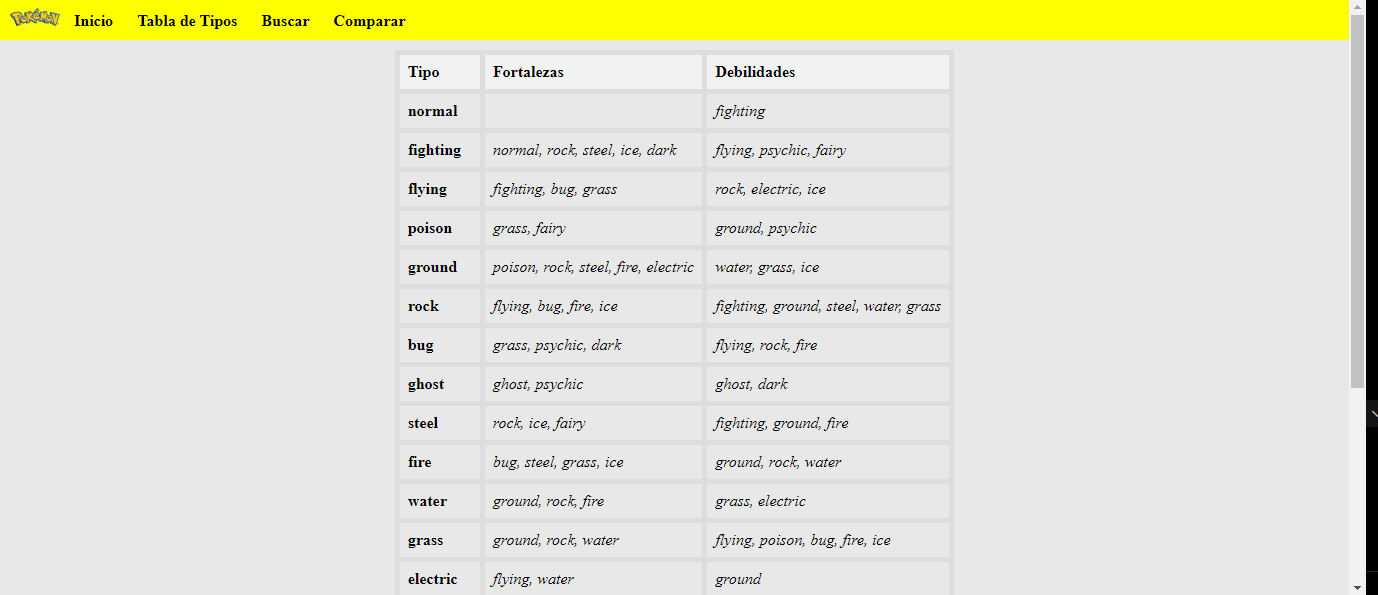
\includegraphics[width=0.5\textwidth]{img/typepage.png}
            \caption{Pagina de Tabla de Tipos}
            \label{figure:typepage}
        \end{figure}
        \vspace{5cm}

        \subsection{Página de Busqueda:}
        La página de busqueda permite encontrar un pokemon por su nombre,filtrar por tipos y por generaciones si el usuario necesita saber cuales son los pokemons tipo fuego de todo el juego o saber cuales pokemons hay en una generación especifica puede filtrar en esta página y encontrarlos.
        \begin{figure}[h]
            \centering
            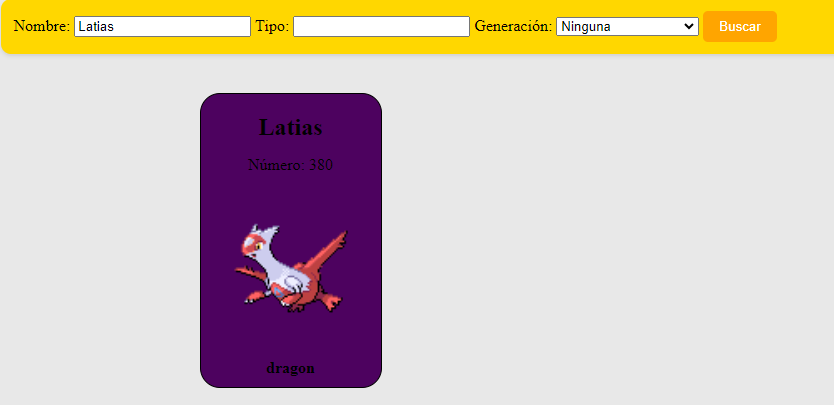
\includegraphics[width=0.3\textwidth]{img/searchpage1.png}
            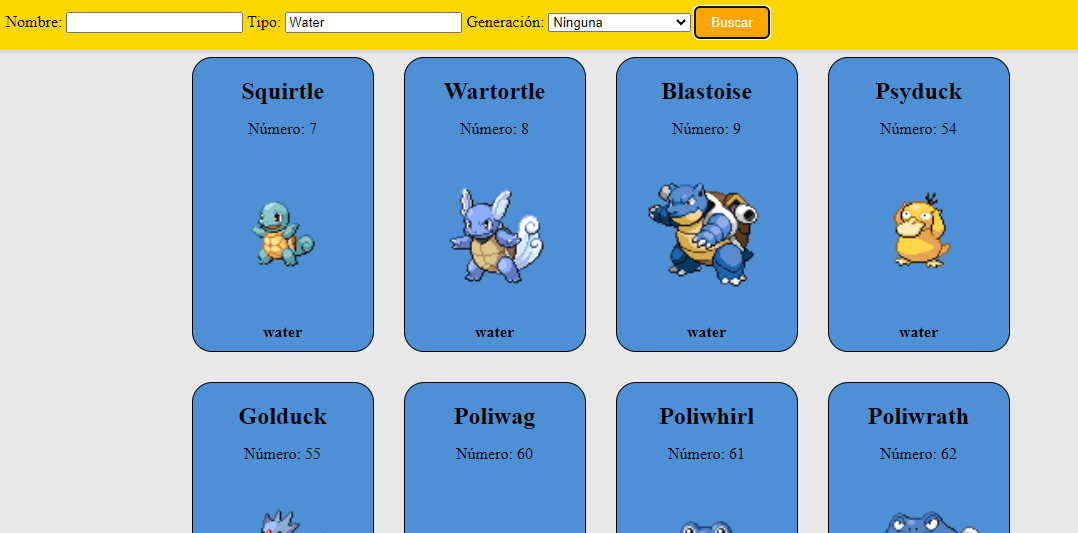
\includegraphics[width=0.3\textwidth]{img/searchpage2.png}
            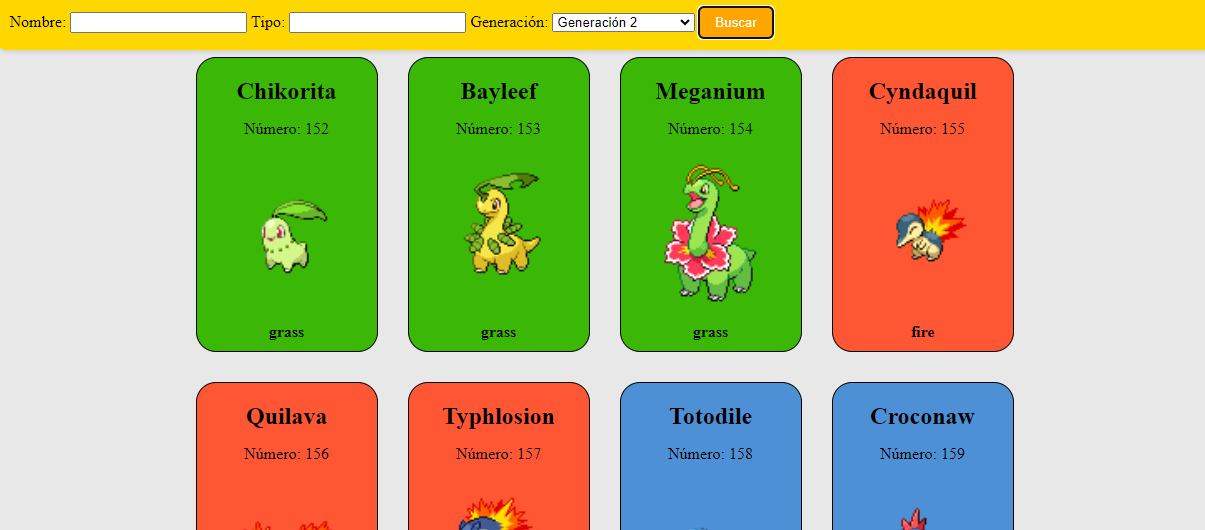
\includegraphics[width=0.3\textwidth]{img/searchpage3.png}
            \caption{Pagina de Busqueda}
            \label{figure:searchpage}
        \end{figure}

        \subsection{Página de Comparación:}
        Este apartado de la aplicación permite que el usuario pueda seleccionar 2 pokemons para compararlos y saber cual ganaría en un posible enfrentamiento esto basandose en su ataque y defensa dentro del juego tomando estos datos desde la API .
        \begin{figure}[h]
            \centering
            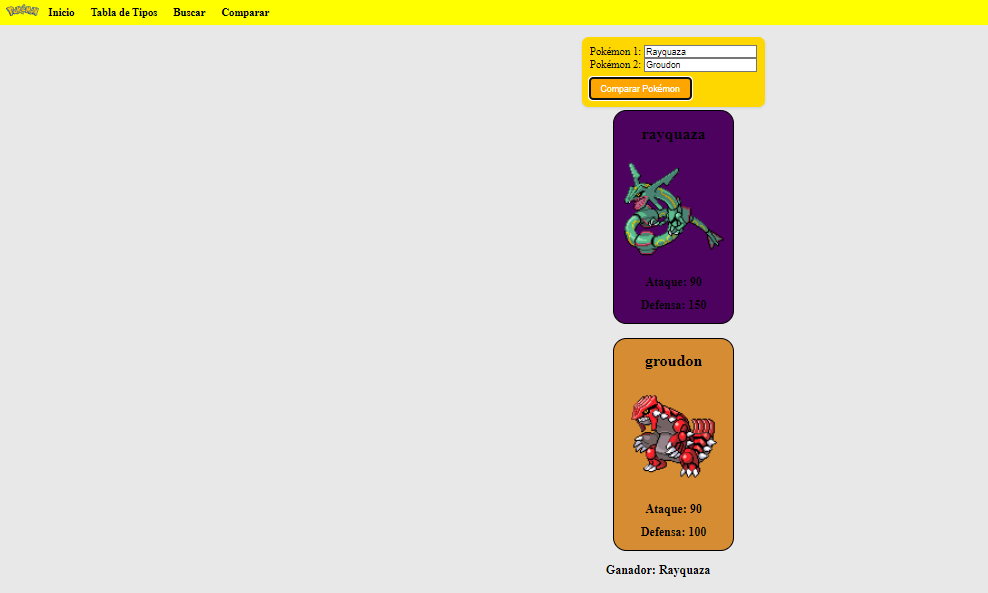
\includegraphics[width=0.5\textwidth]{img/comparepage.png}
            \caption{Pagina de Comparación}
            \label{figure:comparepage}
        \end{figure}
        \vspace{5cm}
        \subsection{Control de versiones: }

        Para mantener un correcto manejo de la aplicación se utilizó un sistema de control de versiones el cual fue GitHub que permite ir trabajando de manera progresiva en el proyecto e ir implementando poco a poco cada una de las funcionalidades del proyecto además que nos permite trabajar con ramas por lo cual se puede estar desarrollando nuevas implementaciones sin afectar la apliación que se encuentra en producción y en caso de causar un daño podríamos volver a un momento de la aplicación donde estaba funcional.
        \begin{figure}[h]
            \centering
            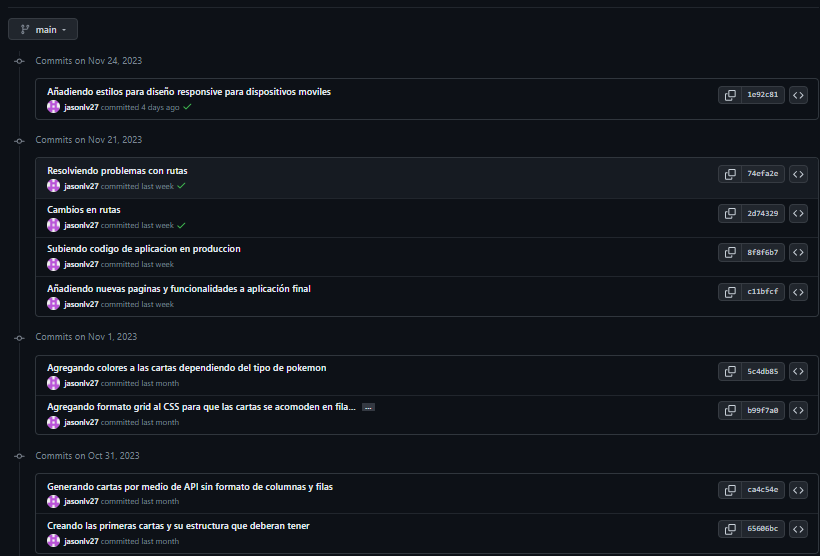
\includegraphics[width=0.5\textwidth]{img/controlversion.png}
            \caption{Control de versiones}
            \label{figure:controlversion}
        \end{figure}

        \subsection{Despliegue:}

        Se despliega la aplicación utilizando un servicio de Github llamado GitHubPages que permite subir el codigó de la aplicación y poder controlarlo desde el repositorio cada vez que se realiza un cambio en la aplicación en la rama main esta cargará el repositorio en GitHubPages y así permite el uso de la aplicación a los usuarios.

        \begin{figure}[h]
            \centering
            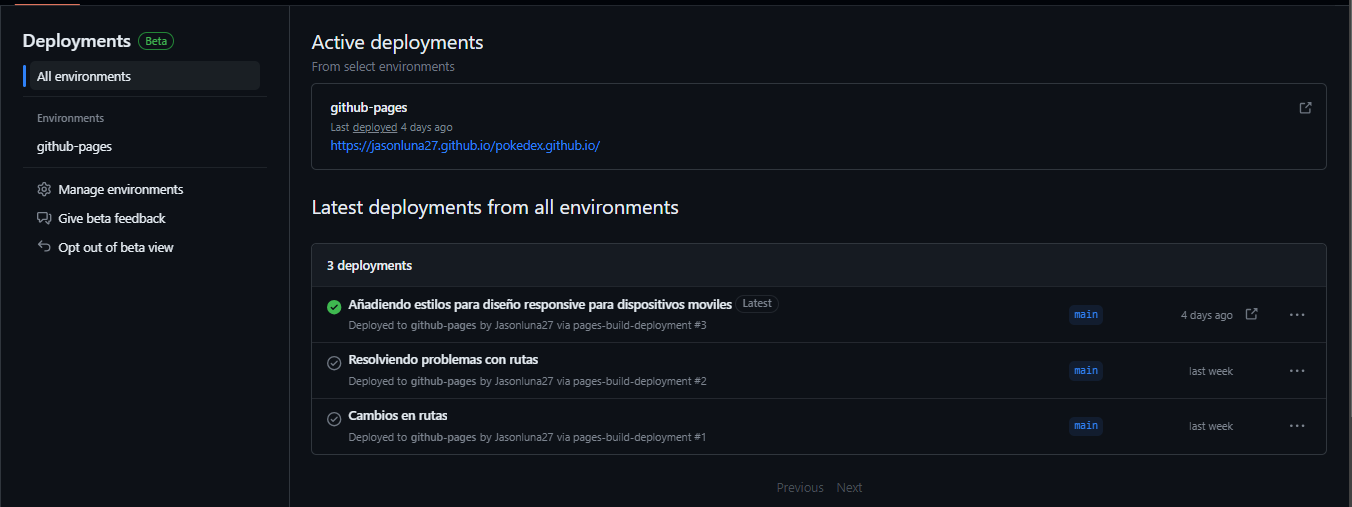
\includegraphics[width=0.5\textwidth]{img/deploy.png}
            \caption{Despliegue}
            \label{figure:Deploy}
        \end{figure}

        \subsection{Diseño Responsive: }
        Se implemento un diseño responsivo esto para que la aplicación funcione en general desde cualquier dispositivo sin que se pierda información o se vea de manera desordenada el contenido de cada una de las páginas para realizar esto se hizo uso de mediaqueries en el codigo CSS.

        \begin{figure}[h]
            \centering
            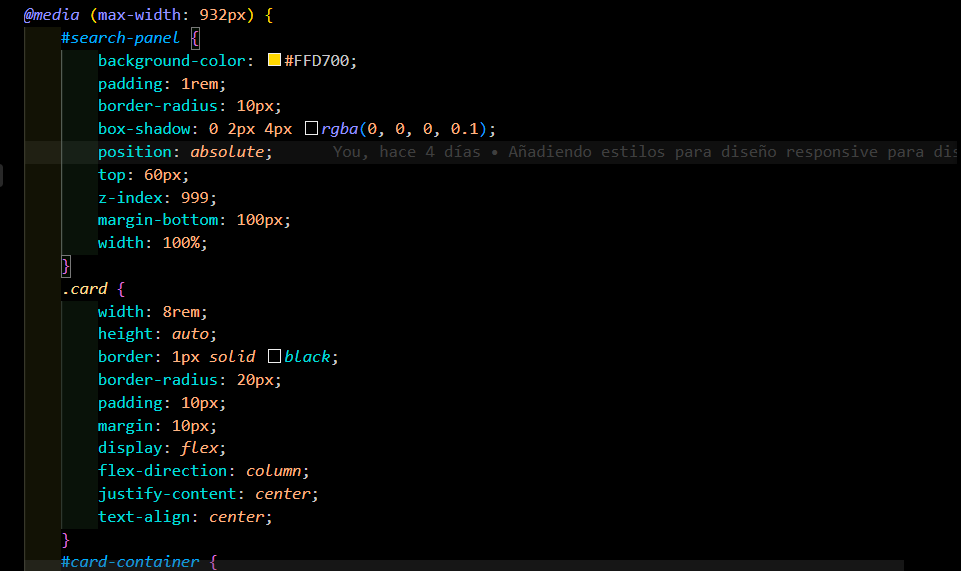
\includegraphics[width=0.5\textwidth]{img/media.png}
            \caption{Diseño responsive}
            \label{figure:responsive}
        \end{figure}
    \section{Conclusiones:}
    \begin{itemize}
        \item Desarrollar un proyecto como este es necesario tener el conocimiento de manejo de APIS, manejo de estilos con CSS e implementación de funciones con JavaScript.
        \item Implementar un framework a esta aplicación si es posible pero se requiere de mas investigación para implementar estas tecnologías.
        \item El uso de control de versiones facilita increiblemente el manejo del proyecto y permite evitar daños en producción.
        \item Hacer uso de mediaqueries permite que la aplicación sea accesible desde dispositivos como computadores,celulares,tabletas sin perder la funcionalidad de la aplicación.
    \end{itemize}
    \vspace{5cm}

    \section{Bibliografía:}
    \begin{thebibliography}{X}
        \bibitem{HTML}
            \textit{HTML: HyperText Markup Language | MDN. (2023, July 17). MDN Web Docs. https://developer.mozilla.org/en-US/docs/Web/HTML}
        \bibitem{CSS}
            \textit{CSS: Cascading Style Sheets | MDN. (2023, July 22). MDN Web Docs. https://developer.mozilla.org/en-US/docs/Web/CSS}
        \bibitem{JavaScript}
            \textit{JavaScript | MDN. (2023, September 25). MDN Web Docs. https://developer.mozilla.org/en-US/docs/Web/JavaScript}
        \bibitem{GitHub}
            \textit{GitHub.com Documentación de la Ayuda. (n.d.). GitHub Docs. https://docs.github.com/es}
        \bibitem{PokeAPI}
            \textit{Documentation - PokéAPI. (n.d.). https://pokeapi.co/docs/v2}
        \bibitem{Repositorio}
            \textit{Repositorio en Github. (2023). Repositorio. https://github.com/Jasonluna27/pokedex.github.io}
        \bibitem{Aplicación}
            \textit{Pokedex. (2023). Aplicación. https://jasonluna27.github.io/pokedex.github.io/}
    \end{thebibliography}

\end{document}